%%%%%%%%%%%%%%%%%%%%%%%%%%%%%%%%%%%%%%%%%%%%%%%%%%%%%%%%%%%%
%%% LIVECOMS ARTICLE TEMPLATE FOR BEST PRACTICES GUIDE
%%% ADAPTED FROM ELIFE ARTICLE TEMPLATE (8/10/2017)
%%%%%%%%%%%%%%%%%%%%%%%%%%%%%%%%%%%%%%%%%%%%%%%%%%%%%%%%%%%%
%%% PREAMBLE
\documentclass[9pt,tutorial]{livecoms}
% Use the 'onehalfspacing' option for 1.5 line spacing
% Use the 'doublespacing' option for 2.0 line spacing
% Use the 'lineno' option for adding line numbers.
% Use the 'pubversion' option for adding the citation and publication information to the document footer, when the DOI is assigned and the article is added to a live issue.
% The 'bestpractices' option for indicates that this is a best practices guide.
% Omit the bestpractices option to remove the marking as a LiveCoMS paper.
% Please note that these options may affect formatting.







\usepackage[T1]{fontenc}
\usepackage[utf8]{inputenc}
\usepackage{lmodern}
\usepackage{verbatim}
\usepackage{graphicx}
\usepackage{amsmath}
\usepackage{amssymb}
\usepackage{amsthm}
\usepackage{tabularx}
\usepackage{multirow}
\usepackage{multicol}
\usepackage{fancyvrb}
\usepackage{float}
\usepackage{listings}
\usepackage{xcolor}
%\usepackage{array}
\usepackage{booktabs}
\usepackage{times}
\usepackage{subcaption}
\usepackage{mathtools}
\usepackage{microtype}
\usepackage{tcolorbox}
\usepackage{newverbs}

\usepackage{listings}

\usepackage[
    type={CC},
    modifier={by-nc-sa},
    version={4.0},
]{doclicense}

\usepackage{wrapfig}
\usepackage{geometry}

\usepackage[version=4]{mhchem}
\usepackage{siunitx}
\DeclareSIUnit\Molar{M}
\usepackage[italic]{mathastext}
\graphicspath{{figures/}}

\definecolor{mylightblue}{RGB}{68.085,183.09,194.055} 
\definecolor{mystrongblue}{RGB}{2.04,74.97,121.89}
\definecolor{myorange}{RGB}{255.0,173.91,72.93}
\definecolor{graytitle}{gray}{0.5}
\definecolor{cverbbg}{gray}{0.93}

%%%%%%%%%%%%%%%%%%%%%%%%%%%%%%%%%%%%%%%%%%%%%%%%%%%%%%%%%%%%
%%% IMPORTANT USER CONFIGURATION
%%%%%%%%%%%%%%%%%%%%%%%%%%%%%%%%%%%%%%%%%%%%%%%%%%%%%%%%%%%%

\newcommand{\versionnumber}{0.1}  % you should update the minor version number in preprints and major version number of submissions.
% Do not add a newline in the next command, no matter how long the repository name is, as it will break the link in the PDF.
\newcommand{\githubrepository}{\url{https://github.com/lammpstutorials/lammpstutorials-article}}  %this should be the main github repository for this article

%%%%%%%%%%%%%%%%%%%%%%%%%%%%%%%%%%%%%%%%%%%%%%%%%%%%%%%%%%%%
%%% ARTICLE SETUP
%%%%%%%%%%%%%%%%%%%%%%%%%%%%%%%%%%%%%%%%%%%%%%%%%%%%%%%%%%%%
\title{A Suite of Tutorials for the LAMMPS-2Aug2023 Simulation Package[Article v\versionnumber]}

\author[1*]{Simon Gravelle}
\affil[1]{University Grenoble Alpes, CNRS, LIPhy, Grenoble, 38000, France}

\corr{simon.gravelle@cnrs.fr}{SG}

\orcid{Simon Gravelle}{0000-0003-2149-6706}

\blurb{This LiveCoMS document is maintained online on GitHub at \githubrepository; to provide feedback, suggestions, or help improve it, please visit the GitHub repository and participate via the issue tracker.}

%%%%%%%%%%%%%%%%%%%%%%%%%%%%%%%%%%%%%%%%%%%%%%%%%%%%%%%%%%%%
%%% PUBLICATION INFORMATION
%%% Fill out these parameters when available
%%% These are used when the "pubversion" option is invoked
%%%%%%%%%%%%%%%%%%%%%%%%%%%%%%%%%%%%%%%%%%%%%%%%%%%%%%%%%%%%
\pubDOI{10.XXXX/YYYYYYY}
\pubvolume{<volume>}
\pubissue{<issue>}
\pubyear{<year>}
\articlenum{<number>}
\datereceived{Day Month Year}
\dateaccepted{Day Month Year}

%%%%%%%%%%%%%%%%%%%%%%%%%%%%%%%%%%%%%%%%%%%%%%%%%%%%%%%%%%%%
%%% ARTICLE START
%%%%%%%%%%%%%%%%%%%%%%%%%%%%%%%%%%%%%%%%%%%%%%%%%%%%%%%%%%%%

\begin{document}

\begin{frontmatter}
\maketitle

\begin{abstract}
This particular document provides a skeleton illustrating key sections for a Tutorial document.
Please see the sample \texttt{sample-document.tex} in \url{github.com/livecomsjournal/article_templates/templates} for additional information on and examples of using the LiveCoMS LaTeX class.
Here we also assume familiarity with LaTeX and knowledge of how to include figures, tables, etc.; if you want examples, see the sample just referenced.

In your work, in this particular slot, please provide an abstract of no more than 250 words.
Your abstract should explain the main contributions of your article, and should not contain any material that is not included in the main text.
Please note that your abstract, plus the authorship material following it, must not extend beyond the title page or modifications to the LaTeX class will likely be needed.
\end{abstract}

\end{frontmatter}




\section{Introduction}

Here you would explain what problem you are tackling and briefly motivate your work.

In this particular template, we have removed most of the usage examples which occur in \texttt{sample-document.tex} to provide a minimal template you can modify; however, we retain a couple of examples illustrating more unusual features of our templates/article class, such as the checklists, and information on algorithms and pseudocode.

Keep in mind, as you prepare your manuscript, that you should plan for a representative image  which will be used to highlight your article on the journal website and publications. Usually, this would be one of your figures, but it must also be uploaded separately upon article submission. We give specific guidelines for this image on the journal website in the section on article submission (see \url{https://livecomsjournal.github.io/authors/policies/index.html#article-submission}).

Additionally, for well-formatted manuscripts, we recommend that you let LaTeX handle figure/table placement for you as much as possible, so please avoid specifying strenuous float instructions like `[h!]` and `[H]` as much as possible.

\subsection{Scope}

Tutorials should endeavor to cover the specific task at hand, and also highlight how the steps might need to be modified (or additional care might need to be taken at particular points) to handle more general cases.

The scope of the tutorial, as well as the expected proficiencies / outcomes for researchers who complete the tutorial, should be clearly defined.
This will often happen in a specific section or subsection in the article itself.

\section{Prerequisites}

Here you would identify prerequisites/background knowledge that are assumed by your work, as well as any software/license requirements.

\subsection{Background knowledge}
Tutorials should clearly define what concepts or abilities researchers will need to complete the tutorial (e.g., some proficiency in Python; experience with Jupyter notebooks; knowledge of classical MD; etc).

\subsection{Software/system requirements}
Tutorials should clearly define what system and/or software requirements the researcher will need to complete the tutorial (e.g., VMD version 1.9 or newer, AMBER, etc.). Tutorials requiring specific software packages must provide instructions and files for the referenced version of the software.

\section{Content and links}

A tutorial will normally draw on additional files and materials; clearly indicate where and how these are available, with links, and how they are being archived for the long-term and maintained so they stay current.
You will likely want to reference your GitHub repository as a central point to access all of this information, and then the GitHub repository may link out to other content as needed.

\subsection{Tutorial 1: Lennard-Jones fluid}
\label{lennard-jones-label}

\begin{figure}
{\centering
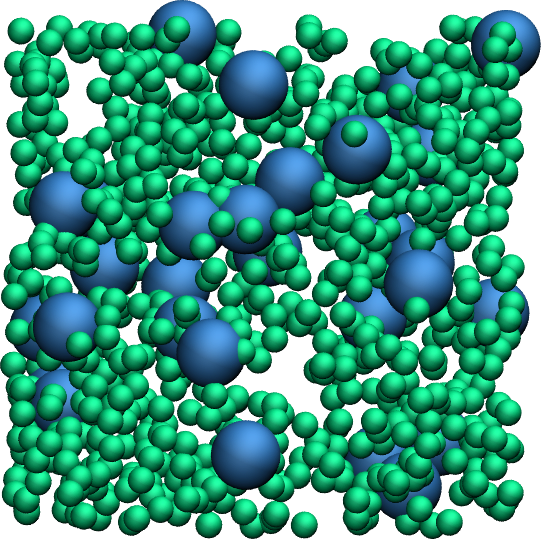
\includegraphics[width=0.55\linewidth]{binary_LJ_fluid}
\caption{Snapshot of the Lennard-Jones fluid made using VMD, with both types of atoms represented as spheres.}}
\label{fig:binary_LJ_fluid}
\end{figure}

\noindent The objective of this tutorial is to perform the simulation of a binary fluid using LAMMPS. The system is a Lennard-Jones fluid made of neutral particles with two different diameters in a cubic box with periodic boundary conditions (Fig.~\ref{fig:binary_LJ_fluid}). The temperature of the system is maintained using a Langevin thermostat \cite{schneider1978molecular}, and basic quantities are extracted from the system, including the potential and kinetic energies. 

\subsubsection{My first input}

\noindent To run a simulation using LAMMPS, one needs to write a series of commands in an input script. For clarity, this script will be divided into five categories which we are going to fill up one by one. Create a folder, call it \textit{my-first-input/}, and then create a blank text file in it called \textit{input.lammps}. Copy the following lines in \textit{input.lammps}, where a line starting with a brace ($\#$) is a comment that is ignored by LAMMPS:
{\small  \begin{verbatim}
# PART A - ENERGY MINIMIZATION
# 1) Initialization
# 2) System definition
# 3) Simulation settings
# 4) Visualization
# 5) Run
\end{verbatim}}
\noindent These five categories are not required in every input script, and should not necessarily be in that exact order. For instance, parts 3 and 4 could be inverted, or part 4 could be omitted. Note however that LAMMPS reads input files from top to bottom, therefore the \textit{Initialization} and \textit{System definition} categories must appear at the top of the input, and the \textit{Run} category at the bottom.

\paragraph{System initialization}
In the first section of the script, called \textit{Initialization}, let us indicate to LAMMPS the most basic information about the simulation, such as:
\begin{itemize}
\item the conditions at the boundaries of the box (e.g. periodic or non-periodic),
\item the type of atoms (e.g. uncharged single dots or spheres with angular velocities).
\end{itemize}
Enter the following lines in \textit{input.lammps}:
{\small \begin{verbatim}
# 1) Initialization
units lj
dimension 3
atom_style atomic
pair_style lj/cut 2.5
boundary p p p
\end{verbatim}}
The first line, \textit{units lj}, indicates that we want to use the system of unit called \textit{LJ}, for Lennard-Jones, for which all quantities are unitless. The second line, \textit{dimension 3}, indicates that the simulation is 3D. The third line, \textit{atom$\_$style atomic}, that the \textit{atomic} style
will be used, therefore each atom is just a dot with a mass. The fourth line, \textit{pair$\_$style lj/cut 2.5}, indicates that atoms will be interacting through a Lennard-Jones potential with a cut-off equal to $r_c = 2.5$ (unitless) \cite{wang2020lennard,fischer2023history}:
$$E_{ij} (r) = 4 \epsilon_{ij} \left[ \left( \dfrac{\sigma_{ij}}{r} \right)^{12} - \left( \dfrac{\sigma_{ij}}{r} \right)^{6} \right], ~ \text{for} ~ r < r_c,$$
where $r$ is the inter-particles distance, $\epsilon_{ij}$ the depth of potential well that sets the interaction strength, and $\sigma_{ij}$ the distance parameter, or particle effective size. Here, the indexes \textit{ij} refer to the particle types \textit{i} and \textit{j}. The last line, \textit{boundary p p p}, indicates that the periodic boundary conditions will be used along all three directions of space (the 3 \textit{p} stand for \textit{x}, \textit{y}, and \textit{z}, respectively).

\paragraph{System definition}
Let us fill the \textit{System definition} category of the input script:
{\small \begin{verbatim}
# 2) System definition
region simulation_box block -20 20 -20 20 -20 20
create_box 2 simulation_box
create_atoms 1 random 1500 341341 simulation_box
create_atoms 2 random 100 127569 simulation_box
\end{verbatim}}
\noindent The first line, \textit{region simulation$\_$box (...)}, creates a region named \textit{simulation$\_$box} that is a block (i.e. a rectangular cuboid) that extends from -20 to 20 (no unit) along all 3 directions of space. The second line, \textit{create$\_$box 2 simulation$\_$box}, creates a simulation box based on the region \textit{simulation$\_$box} with \textit{2} types of atoms. The third line, \textit{create$\_$atoms (...)} creates 1500 atoms of type 1 randomly within the region \textit{simulation$\_$box}. The integer \textit{341341} is a seed that can be changed in order to create different
initial conditions for the simulation. The fourth line creates 100 atoms of type 2.

\paragraph{Simulation Settings}
Let us fill the \textit{Simulation Settings} category section of the \textit{input} script:
{\small \begin{verbatim}
# 3) Simulation settings
mass 1 1
mass 2 1
pair_coeff 1 1 1.0 1.0
pair_coeff 2 2 0.5 3.0
\end{verbatim}}
The two first commands, \textit{mass (...)}, attribute a mass equal to 1 (unitless) to both atoms of type 1 and 2. Alternatively, one could have written these two commands into one single line: \textit{mass $\star 1$}, where the star symbol means \textit{all} the atom types of the simulation.  The third line, \textit{pair$\_$coeff 1 1 1.0 1.0}, sets the Lennard-Jones coefficients for the interactions between atoms of type 1, respectively the energy parameter $\epsilon_{11} = 1.0$ and the distance parameter $\sigma_{11} = 1.0$. Similarly, the last line sets the Lennard-Jones coefficients for the interactions between atoms of type 2, $\epsilon_{22} = 0.5$, and $\sigma_{22} = 3.0$. By default, LAMMPS calculates the cross coefficients between the different atom types using geometric average: $\epsilon_{ij} = \sqrt{\epsilon_{ii} \epsilon_{jj}}$, $\sigma_{ij} = \sqrt{\sigma_{ii} \sigma_{jj}}$. 


\paragraph{Energy minimization}
The system is now fully parametrized. Let us fill the two last remaining sections by adding the following lines to \textit{input.lammps}:
\begin{verbatim}
# 4) Visualization
thermo 10
thermo_style custom step temp pe ke etotal press

# 5) Run
minimize 1.0e-4 1.0e-6 1000 10000
\end{verbatim}
The \textit{thermo} command asks LAMMPS to print thermodynamic information (e.g. temperature, energy) in the terminal every given number of steps, here 10 steps. The \textit{thermo$\_$style custom} requires LAMMPS to print the system temperature (\textit{temp}), potential energy (\textit{pe}), kinetic energy (\textit{ke}), total energy (\textit{etotal}), and pressure (\textit{press}). Finally, the \textit{minimize} line asks LAMMPS to perform an energy minimization of the system. By default, LAMMPS uses the conjugate gradient (CG) algorithm \cite{hestenes1952methods}.

Run the simulation by typing in a terminal:
\begin{verbatim}
lmp -in input.lammps
\end{verbatim}
where the command \textit{lmp} is linked to a compiled version of LAMMPS. As the simulation progresses, the potential energy can be seen to decrease from a large positive value to to a negative value. The initially large and positive value of the potential energy was expected because the atoms have been created at random positions within the simulation box and some of them are probably overlapping, resulting in a large initial energy which is the consequence of the repulsive part of the Lennard-Jones interaction potential. As the energy minimization progresses, the energy rapidly decreases and reaches a negative value, indicating that the atoms have been displaced at reasonable distances from each other.

\paragraph{Molecular dynamics}
The system is now ready. Let us continue filling up the input script and adding commands to perform a molecular dynamics simulation that will start from the final state of the previous energy minimization step. In the same input script, after the \textit{minimization} command, add the following
lines:
\begin{verbatim}
# PART B - MOLECULAR DYNAMICS
# 4) Visualization
thermo 50
\end{verbatim}
Since LAMMPS reads the input from top to bottom, these lines will be executed after the energy minimization. There is no need to re-initialize or re-define the system. The \textit{thermo} command is called a second time within the same input, so the previously entered value of 10 will be replaced by
the value of 50 as soon as \textit{PART B} starts. Then, let us add a second \textit{Run} section:
\begin{verbatim}
# 5) Run
fix mynve all nve
fix mylgv all langevin 1.0 1.0 0.1 1530917
timestep 0.005
run 10000
\end{verbatim}
The \textit{fix nve} is used to update the positions and the velocities of the atoms in the group \textit{all} at every step. The group \textit{all} is a default group that contains every atom. The second fix applies a Langevin thermostat to the atoms of the group \textit{all}, with a desired initial temperature of 1.0 (unitless), and a final temperature of 1.0 as well \cite{schneider1978molecular}. A \textit{damping} parameter of 0.1 is used. The \textit{damping} parameter determines how rapidly the temperature is relaxed to its desired value. The number \textit{1530917} is a seed, you can change it to perform statistically independent simulations. Finally, the last two lines set the value of the \textit{timestep} and the number of steps for the *run*, respectively, corresponding to a total duration of 50 (unitless).

Run the simulation again using LAMMPS. {\color{red}From the log file}, one can see that the temperature \textit{Temp} starts from 0, but rapidly reaches the requested value and stabilize itself near $T=1$ (unitless). \vspace{0.25cm} \noindent From what has been printed in the \textit{log} file, one can plot the potential energy ($p_\text{e}$) and the kinetic energy ($k_\text{e}$) of the system over time {\color{red}(see the figure below)}.

{\color{red}Figure: a) The potential energy ($p_\text{e}$) rapidly decreases during energy minimization (orange). Then, after the molecular dynamics simulation starts, $p_\text{e}$ increases until it reaches a plateau value of about -0.25 (blue). b) The kinetic energy ($k_\text{e}$) is equal to zero during energy minimization, then increases during molecular dynamics until it reaches a plateau value of about 1.5.}

\paragraph{Trajectory visualization}

The simulation is running well, but we would like to visualize the trajectories of the atoms. To do so, we first need to print the positions of the atoms in a file at a regular interval. Add the following command to the \textit{input.lammps} file, in the \textit{Visualization} section of \textit{PART B}:
\begin{verbatim}
dump mydmp all atom 100 dump.lammpstrj
\end{verbatim}
Run the \textit{input.lammps} using LAMMPS again. A file named \textit{dump.lammpstrj} must appear within \textit{my-first-input/}. A \textit{.lammpstrj} file can be opened using VMD. {\color{red}With Ubuntu/Linux}, you can simply execute in the terminal:
\begin{verbatim}
vmd dump.lammpstrj
\end{verbatim}
Otherwise, you can open VMD and import the \textit{dump.lammpstrj} file manually using \textit{File -> New molecule}.
By default, you should see a cloud of lines, but you can improve the representation (see this {\color{red}VMD tutorial} for basic instructions).

{\color{red}Figure: View of a slice of the system using VMD, with both types of atoms represented as spheres. See the corresponding \href{https://youtu.be/vdSIJM5fVJE}{video}.}


\subsubsection{Improving the script}

Let us improve the input script and perform slightly more advanced operations, such as imposing a specific initial
positions to the atoms, and restarting the simulation from a previously saved configuration. 

\paragraph{Control the initial atom positions}
\noindent Create a new folder next to \textit{my-first-input/}, and call it \textit{improved-input/}. Then, create a new input file within \textit{improved-input/} and call it \textit{input.min.lammps}. Similarly to what has been done previously, copy the following lines into \textit{input.min.lammps}:
\begin{verbatim}
# 1) Initialization
units lj
dimension 3
atom_style atomic
pair_style lj/cut 2.5
boundary p p p
\end{verbatim}
To create the atoms of types 1 and 2 in two separate regions, let us create three separate regions: A cubic region for the simulation box and two additional regions for placing the atoms:
\begin{verbatim}
# 2) System definition
region simulation_box block -20 20 -20 20 -20 20
create_box 2 simulation_box
region cylinder_in cylinder z 0 0 10 INF INF side in
region cylinder_out cylinder z 0 0 10 INF INF side out
create_atoms 1 random 1000 341341 cylinder_out
create_atoms 2 random 150 127569 cylinder_in
\end{verbatim}
The \textit{side in} and \textit{side out} keywords are used to define regions that are respectively inside and outside of the cylinder of radius 10. Then, copy similar lines as previously into \textit{input.min.lammps}:
\begin{verbatim}
# 3) Simulation settings
mass 1 1
mass 2 1
pair_coeff 1 1 1.0 1.0
pair_coeff 2 2 0.5 3.0

# 4) Visualization
thermo 10
thermo_style custom step temp pe ke etotal press
dump mydmp all atom 10 dump.min.lammpstrj

# 5) Run
minimize 1.0e-4 1.0e-6 1000 10000
write_data minimized_coordinate.data
\end{verbatim}
The main novelty, compared to the previous input script, is the \textit{write$\_$data} command. This command is used to print the final state of the simulation in a file named \textit{minimized$\_$coordinate.data}. Note that the \textit{write$\_$data} command is placed after the \textit{minimize} command. This \textit{.data} file will be used later to restart the simulation from the final state of the energy minimization step.

Run the \textit{input.min.lammps} script using LAMMPS. A new dump file named \textit{dump.min.lammpstrj} will appear in the folder, allowing you to visualize
the atom's trajectories during minimization. In addition, a file named \textit{minimized$\_$coordinate.data} will be created. If you open \textit{minimized$\_$coordinate.data} with a text editor, you can see that it contains all the information necessary to restart the simulation, such as the number of atoms and the box size, the \textit{masses}, the \textit{pair$\_$coeffs}:
\begin{verbatim}
1150 atoms
2 atom types

-20 20 xlo xhi
-20 20 ylo yhi
-20 20 zlo zhi

Masses

1 1
2 1

Pair Coeffs # lj/cut

1 1 1
2 0.5 3
(...)
\end{verbatim}
The \textit{minimized$\_$coordinate.data} file also contains the final positions of the atoms:
\begin{verbatim}
(...)
Atoms # atomic

970 1 4.4615279184230525 -19.88248310680258 -19.497251754277872 0 0 0
798 1 1.0773937287460968 -17.57843015813612 -19.353475858951473 0 0 0
21 1 -17.542385434367777 -16.647460269156497 -18.93914807895693 0 0 0
108 1 -15.96241088290946 -15.956274144833264 -19.016419910024062 0 0 0
351 1 0.08197850837343444 -16.852380573900156 -19.28249747472579 0 0 0
402 1 -5.270160783673711 -15.592291204068946 -19.6382667867645 0 0 0
(...)
\end{verbatim}
The first five columns of the \textit{Atoms} section correspond (from left to right) to the atom indexes (from 1 to the total number of atoms, 1150), the atom types (1 or 2 here), and the atoms positions $x$, $y$, $z$. The last three columns are image flags that keep track of which atoms crossed the periodic boundary.

\paragraph{Restarting from a saved configuration}
Let us create a new input file and start a molecular dynamics simulation directly from the previously saved configuration. Within \textit{improved-input/}, create a new file named \textit{input.md.lammps} and copy the same lines as previously:
\begin{verbatim}
# 1) Initialization
units lj
dimension 3
atom_style atomic
pair_style lj/cut 2.5
boundary p p p
\end{verbatim}
Now, instead of creating a new region and adding atoms to it, we can simply add the following command:
\begin{verbatim}
# 2) System definition
read_data minimized_coordinate.data
\end{verbatim}
By visualizing the previously generated \textit{dump.min.lammpstrj} file, you may have noticed that some atoms have moved from one region to the other during minimization. To start the simulation from a clean slate, with only atoms of type 2 within the cylinder and atoms of type
1 outside the cylinder, let us delete the misplaced atoms by adding the following commands to \textit{input.md.lammps}:
\begin{verbatim}
read_data minimized_coordinate.data
region cylinder_in cylinder z 0 0 10 INF INF side in
region cylinder_out cylinder z 0 0 10 INF INF side out
group group_type_1 type 1
group group_type_2 type 2
group group_region_in region cylinder_in
group group_region_out region cylinder_out
group group_type_1_in intersect group_type_1 group_region_in
group group_type_2_out intersect group_type_2 group_region_out
delete_atoms group group_type_1_in
delete_atoms group group_type_2_out
\end{verbatim}
The two first \textit{region} commands recreate the previously defined regions, which is necessary since regions are not saved by the \textit{write$\_$data} command. The first two \textit{group} commands create atom groups based on their types. The next two \textit{group} commands create atom groups based on their
positions at the beginning of the simulation, i.e. when the commands are being read by LAMMPS. The last two \textit{group} commands create atom groups based on the intersection between the previously defined groups. Finally, the two \textit{delete$\_$atoms} commands delete the atoms of type 1 that are located within the cylinder, as well as the atoms of type 2 that are located outside the cylinder, respectively. 

{\color{red}When you run the \textit{input.md.lammps} input using LAMMPS, you can see in the \textit{log} file how many atoms are in each group, and how many atoms have been deleted:}
\begin{verbatim}
1000 atoms in group group_type_1
150 atoms in group group_type_2
149 atoms in group group_region_in
1001 atoms in group group_region_out
0 atoms in group group_type_1_in
1 atoms in group group_type_2_out
Deleted 0 atoms, new total = 1150
Deleted 1 atoms, new total = 1149
\end{verbatim}
Add the following lines to \textit{input.md.lammps}. Note the absence of \textit{Simulation settings} section, because the settings are taken from the \textit{.data} file.
\begin{verbatim}
# 4) Visualization
thermo 1000
dump mydmp all atom 1000 dump.md.lammpstrj
\end{verbatim}
Let us extract the number of atoms of each type inside the cylinder as a function of time, by adding the following commands to \textit{input.md.lammps}:
\begin{verbatim}
variable number_type1_in equal count(group_type_1,cylinder_in)
variable number_type2_in equal count(group_type_2,cylinder_in)
fix myat1 all ave/time 10 200 2000 v_number_type1_in &
    file output-population1vstime.dat
fix myat2 all ave/time 10 200 2000 v_number_type2_in &
    file output-population2vstime.dat
\end{verbatim}
The 2 \textit{variables} are used to count the number of atoms of a specific group in the \textit{cylinder$\_$in} region. The two \textit{fix ave/time} are calling the previously defined variables and are printing their values into text files. By using \textit{10 200 2000}, variables are evaluated every 10 steps, averaged 200 times, and printed in the \textit{.dat} files every 2000 steps.

Let us also extract the coordination number per atom between atoms of type 1 and 2, i.e. the average number of atoms of type 2 in the vicinity of the atoms of type 1. This coordination number will be used as an indicator of the degree of mixing of our binary mixture. Add the following lines into \textit{input.md.lammps}:
\begin{verbatim}
compute coor12 group_type_1 coord/atom cutoff 2.0 group group_type_2
compute sumcoor12 all reduce ave c_coor12
fix myat3 all ave/time 10 200 2000 &
    c_sumcoor12 file coordinationnumber12.dat
\end{verbatim}
The \textit{compute ave} is used to average the per atom coordination number that is calculated by the \textit{coord/atom} compute. This averaging is necessary as \textit{coord/atom} returns an array where each value corresponds to a certain couple of atoms i-j. Such an array can't be printed by \textit{fix ave/time}. Finally, let us complete the script by adding the following lines to \textit{input.md.lammps}:
\begin{verbatim}
# 5) Run
velocity all create 1.0 4928459 mom yes rot yes dist gaussian
fix mynve all nve
fix mylgv all langevin 1.0 1.0 0.1 1530917 zero yes
timestep 0.005
run 300000
write_data mixed.data
\end{verbatim}
There are a few differences from the previous simulation. First, the \textit{velocity create} command attributes an initial velocity to every atom.
The initial velocity is chosen so that the average initial temperature is equal to 1 (unitless). The additional keywords ensure that no linear momentum (\textit{mom yes}) and no angular momentum (\textit{rot yes}) are given to the system and that the generated velocities are distributed as a Gaussian. Another improvement is the \textit{zero yes} keyword in the Langevin thermostat, which ensures that the total random force is equal to zero.
Run \textit{input.md.lammps} using LAMMPS. Open the \textit{dump.md.lammpstrj} using VMD to observe the mixing of the two populations as the time evolves (Fig.\,\ref{fig:evolution-population}). The generated \textit{.dat} files indicate the number of atoms in each region as a function time (Fig.\,\ref{fig:mixing}\,a). In addition, as the mixing progresses, the calculated coordination number increases from about $0.01$ to $0.35$ (Fig.\,\ref{fig:mixing}\,b).

\begin{figure}
\centering
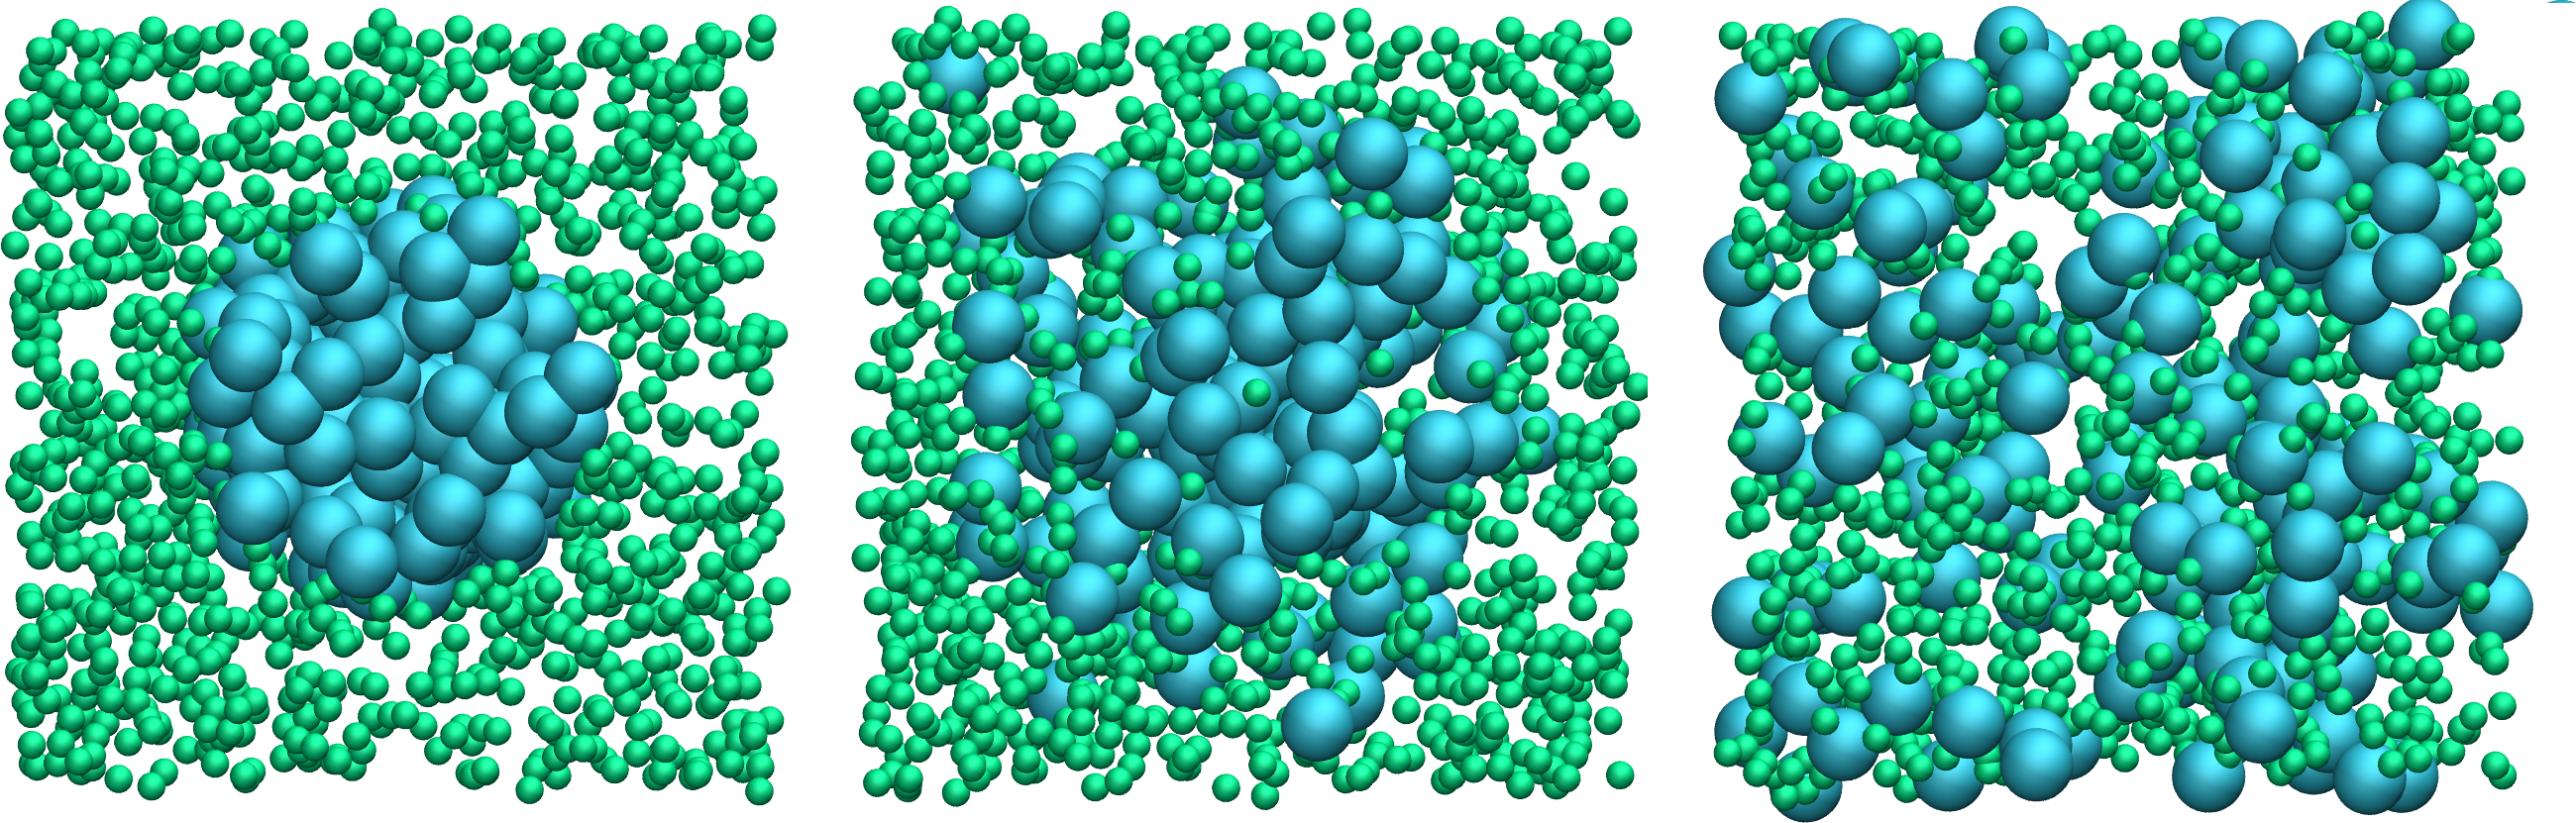
\includegraphics[width=\linewidth]{evolution}
\caption{Evolution of the system during mixing.}
\label{fig:evolution-population}
\end{figure}

\begin{figure}
\centering
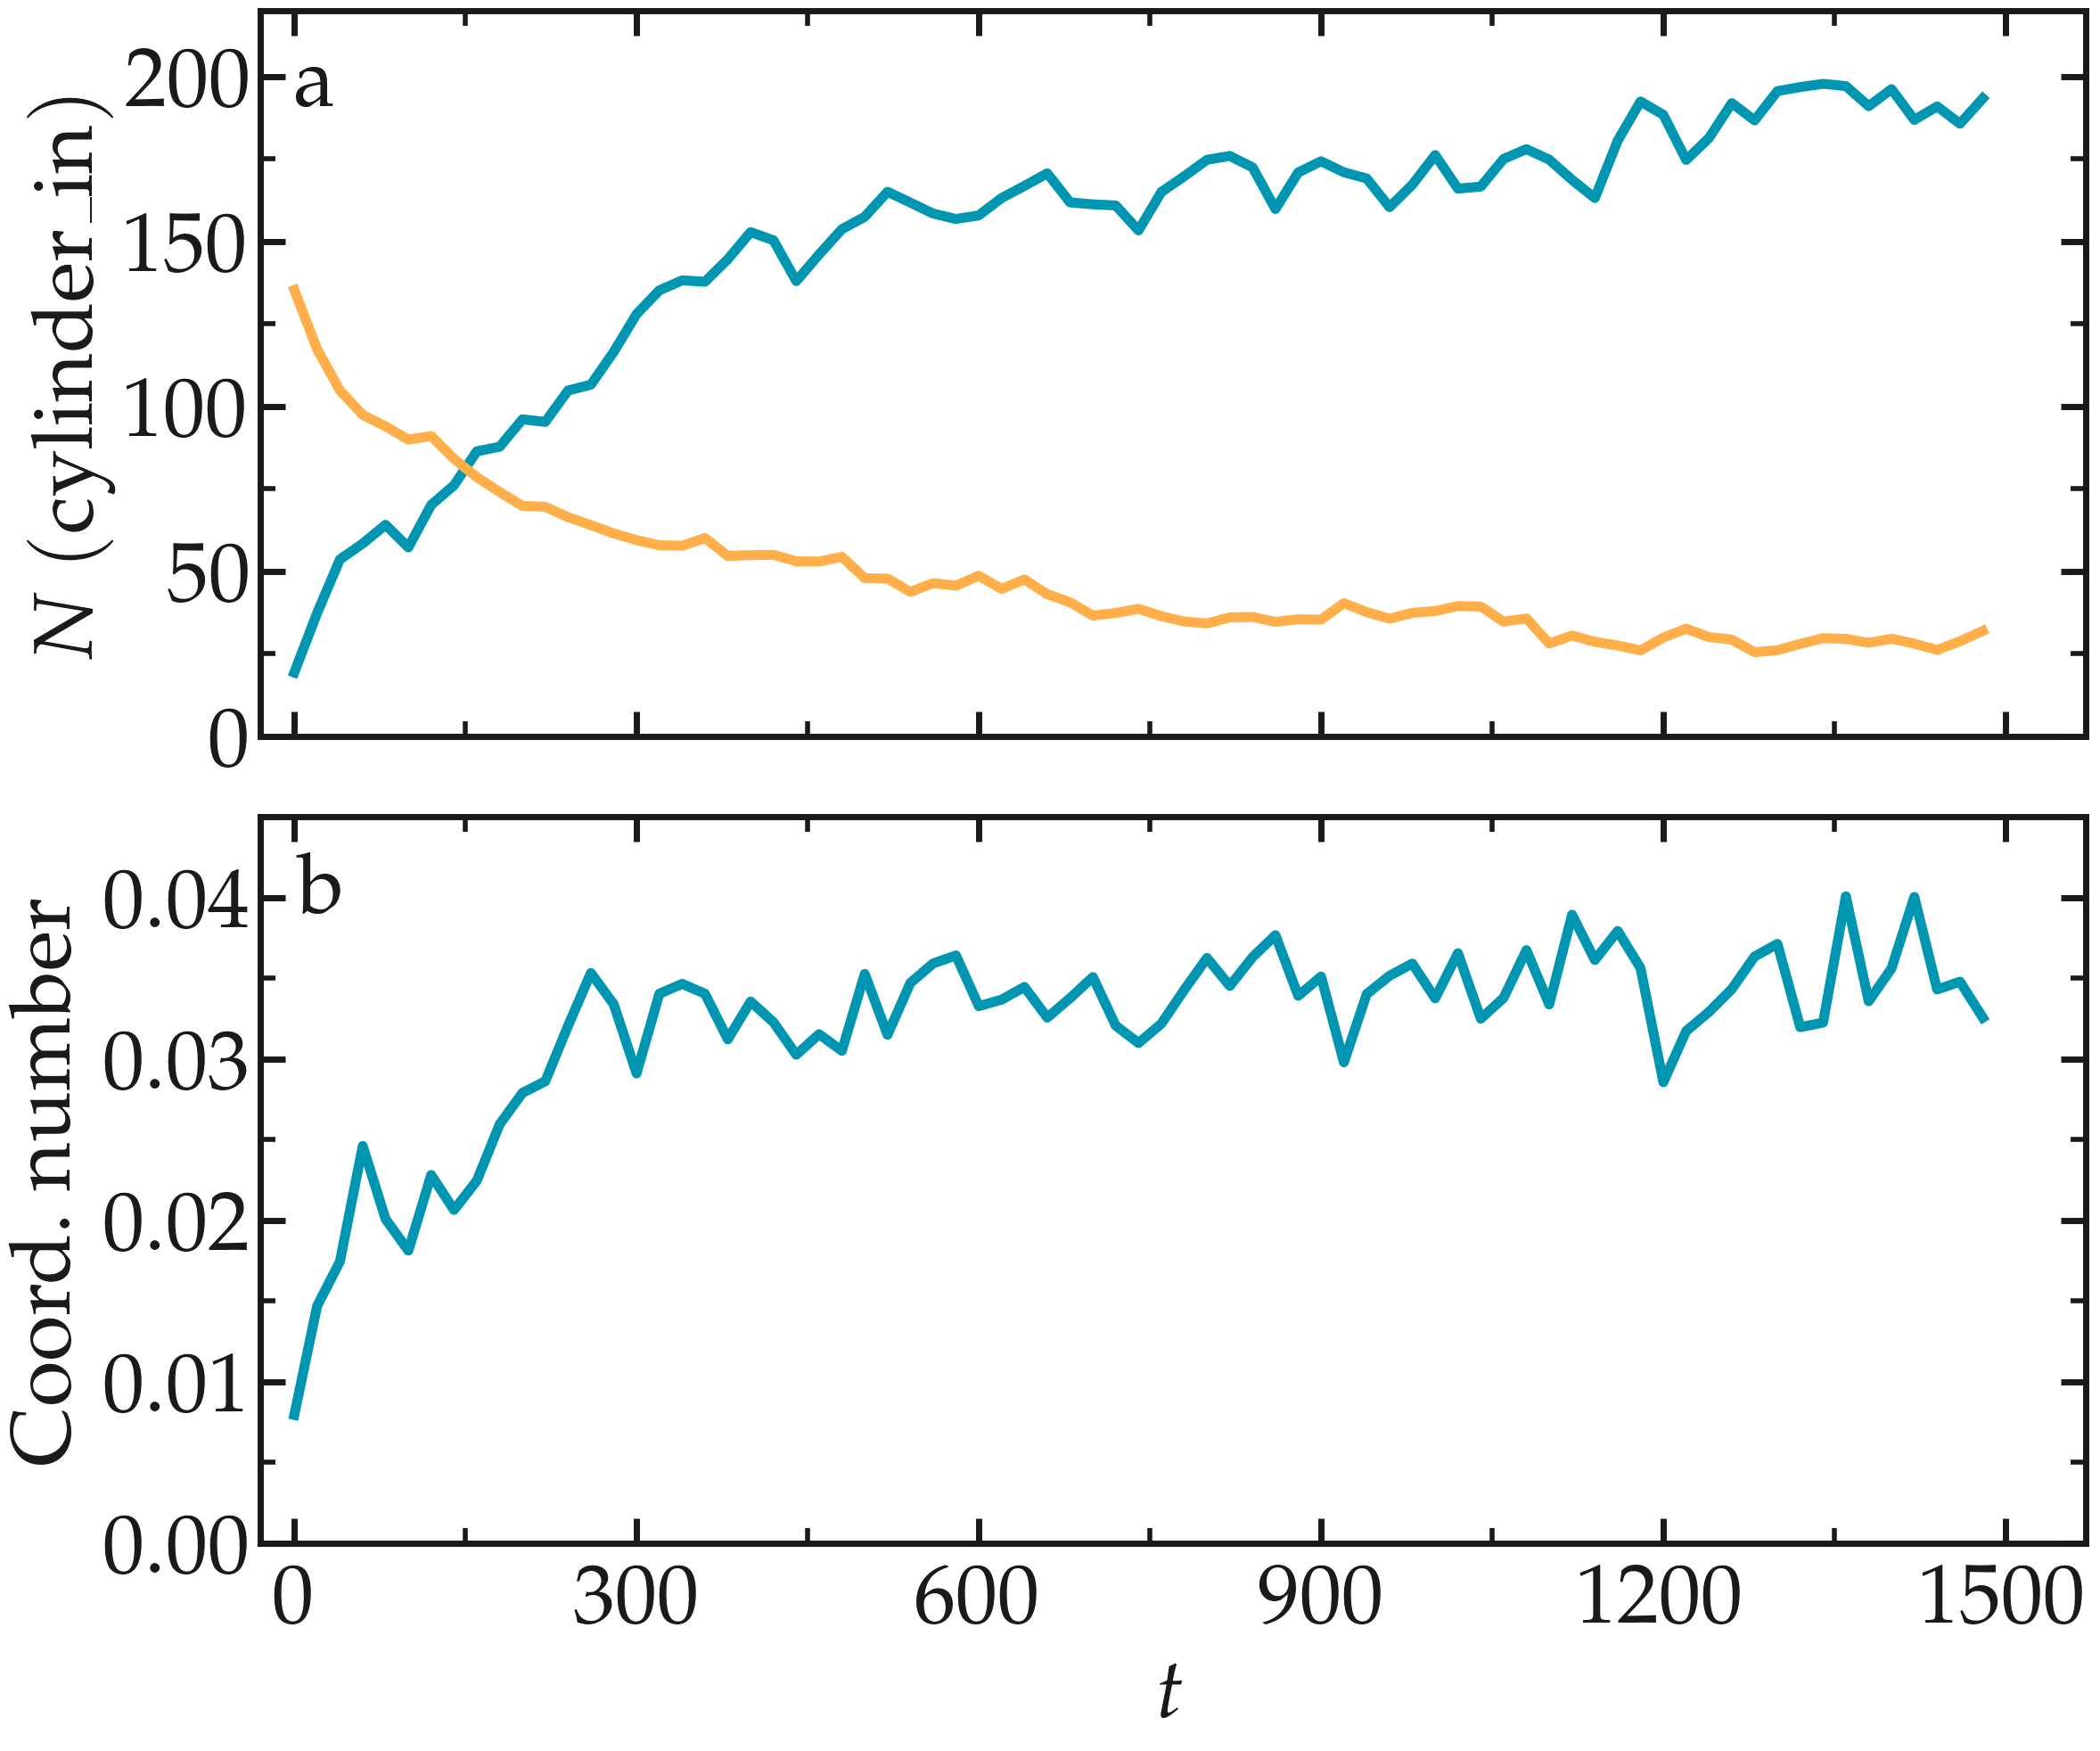
\includegraphics[width=\linewidth]{mixing}
\caption{Evolution of the number $N$ of atoms within the \textit{cylinder$\_$in} region as a function of the time $t$ (a),
and evolution of the coordination number (b).}
\label{fig:mixing}
\end{figure}


\subsection{Tutorial 2: Pulling on a carbon nanotube}
\label{carbon-nanotube-label}

\begin{figure}
{\centering
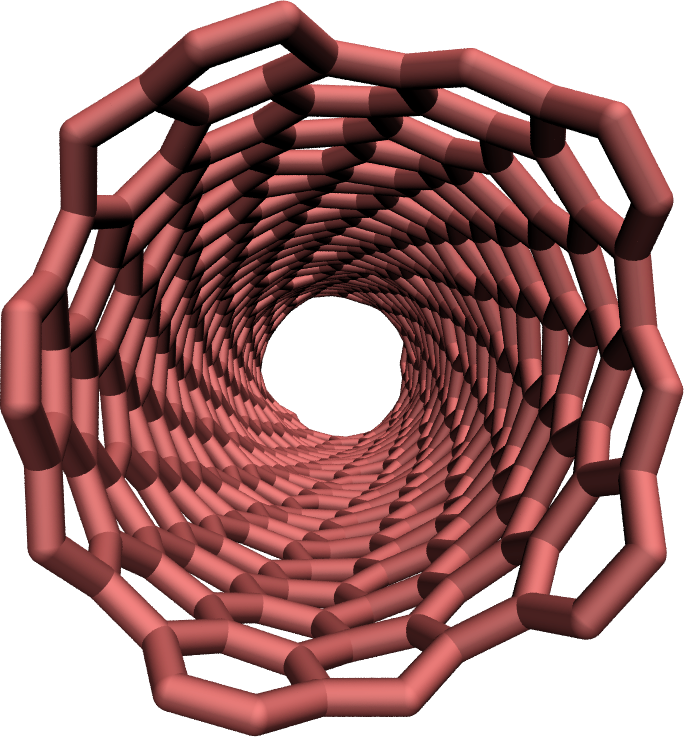
\includegraphics[width=0.55\linewidth]{CNT}
\caption{Snapshot of the carbon nanotube (CNT) made using VMD.}}
\label{fig:CNT}
\end{figure}

\vspace{0.25cm} \noindent The objective of this tutorial is to impose the deformation of a carbon nanotube (CNT) using LAMMPS. In this tutorial, a small carbon nanotube (CNT) is simulated within an empty box using LAMMPS (Fig.\,\ref{fig:CNT}). An external forcing is imposed on the CNT, and its deformation is measured with time. The difference between classical and reactive force fields
is illustrated through this tutorial. With a classical force field, the bonds between atoms are unbreakable. With the reactive force field (named AIREBO \cite{stuart2000reactive}), the breaking of the chemical bonds is possible when the imposed deformation is strong enough.

\subsubsection{Unbreakable bonds}
\noindent With most classical molecular dynamics force fields, the chemical bonds between the atoms are set at the start of the simulation. Regardless of the forces applied to the atoms during the simulations, the bonds remain intact. The bonds between neighbor atoms typically consist of springs with given equilibrium distances $r_0$ and a constant $k_b$: $U_b = k_b \left( r - r_0 \right)^2$.
Additionally, angular and dihedral constraints are usually applied to maintain the relative orientations of neighbor atoms. 

Download directly the CNT topology by clicking \href{https://lammpstutorials.github.io/lammpstutorials-inputs/level1/breaking-a-carbon-nanotube/unbreakable-bonds/cnt_molecular.data}{here}. It was created using VMD and TopoTools \cite{kohlmeyer2017topotools}, and contains information about the positions of the carbon atoms, as well as the
identity of the atoms that are linked by \textit{bonds}, \textit{angles}, \textit{dihedrals},
and \textit{impropers} constraints. Save the \textit{cnt$\_$molecular.data} file
in a folder named \textit{unbreakable-bonds/}.

\paragraph{The LAMMPS input}
Create a new text file within \textit{unbreakable-bonds/} and name it \textit{input.lammps}. Copy the following lines in it:
\begin{verbatim}
variable T equal 300

units real
atom_style molecular
boundary f f f
pair_style lj/cut 14

bond_style harmonic
angle_style harmonic
dihedral_style opls
improper_style harmonic

special_bonds lj 0.0 0.0 0.5

read_data cnt_molecular.data
\end{verbatim}
The chosen unit system is \textit{real} (therefore distances are in Ångstrom, time in femtosecond), the \textit{atom$\_$style} is molecular (therefore atoms are dots that can be bonded with each other), and the boundary conditions are fixed. The boundary conditions do not matter here, as the box boundaries were placed far from the CNT. 

Just like in the previous tutorial, \hyperref[lennard-jones-label]{Lennard Jones fluid}, the pair style is \textit{lj/cut} (i.e. a Lennard-Jones potential with a short-range cutoff) with parameter 14, which means that only the atoms closer than 14 Ångstroms from each other interact through a Lennard-Jones potential. The \textit{bond$\_$style}, \textit{angle$\_$style}, \textit{dihedral$\_$style}, and \textit{improper$\_$style} commands specify the different potentials used to restrain the relative positions of the atoms. For more details about the potentials used here, you can have a look at the LAMMPS website. The \textit{special$\_$bonds} command sets the weighting factors for the Lennard-Jones interaction between atoms directly connected by a bond, separated by two bonds, and separated by three bonds, respectively. The last command, \textit{read$\_$data}, imports the \textit{cnt$\_$molecular.data} file previously generated with VMD, which contains the information about the box size, atom positions, etc.

We need to specify the parameters of both bonded and non-bonded potentials. Here, the parameters are taken from the OPLS-AA (Optimised Potentials for Liquid Simulations-All-Atom) force field \cite{jorgensenDevelopmentTestingOPLS1996}. Create a new text file in the \textit{unbreakable-bonds/} folder and name it \textit{parm.lammps}. Copy the following lines in it:
\begin{verbatim}
pair_coeff 1 1 0.066 3.4
bond_coeff 1 469 1.4
angle_coeff 1 63 120
dihedral_coeff 1 0 7.25 0 0
improper_coeff 1 5 180
\end{verbatim}
The \textit{pair$\_$coeff} command sets the parameters for the non-bonded Lennard-Jones interaction $\epsilon_{11} = 0.066 \, \text{kcal/mol}$ and $\sigma_{11} = 3.4 \, \text{Å}$ for the only type of atom of the simulation; the carbon atom of type 1.  The \textit{bond$\_$coeff} provides the equilibrium distance $r_0= 1.4 \, \text{Å}$ as well as the spring constant $k_b = 469 \, \text{kcal/mol/Å}^2$ for the harmonic potential imposed between two neighboring carbon atoms, where the potential is $U_b = k_b ( r - r_0)^2$. The
\textit{angle$\_$coeff} gives the equilibrium angle $\theta_0$ and constant for the potential between three neighbor atoms :
$U_\theta = k_\theta ( \theta - \theta_0)^2$. The \textit{dihedral$\_$coeff} and \textit{improper$\_$coeff} gives the potential for the constraints between 4 atoms. The file \textit{parm.lammps} is included in the simulation by adding the following line to the \textit{input.lammps} file:
\begin{verbatim}
include parm.lammps
\end{verbatim}


\paragraph{Prepare initial state}
Before starting the molecular dynamics simulation, let us make sure that we start from a clean initial state
by recentering the CNT at the origin (0, 0, 0). In addition, let us make sure that the box boundaries are symmetric with respect to (0, 0, 0), which is not initially the case, as seen in \textit{cnt$\_$molecular.data}:
\begin{verbatim}
-40.000000 40.000000  xlo xhi
-40.000000 40.000000  ylo yhi
-12.130411 67.869589  zlo zhi
\end{verbatim}
Let us recenter the CNT by adding the following lines to \textit{input.lammps}:
\begin{verbatim}
group carbon_atoms type 1
variable carbon_xcm equal -1*xcm(carbon_atoms,x)
variable carbon_ycm equal -1*xcm(carbon_atoms,y)
variable carbon_zcm equal -1*xcm(carbon_atoms,z)
displace_atoms carbon_atoms &
    move ${carbon_xcm} ${carbon_ycm} ${carbon_zcm}
\end{verbatim}
The first command includes all the atoms of type 1 (i.e. all the atoms here) in a group named \textit{carbon$\_$atoms}. 
The 3 variables, \textit{carbon$\_$xcm}, \textit{carbon$\_$ycm}, and \textit{carbon$\_$zcm} are used to measure
the current position of the group \textit{carbon$\_$atoms} along all 3 directions, respectively. Then, the \textit{displace$\_$atoms} 
command move the group \textit{carbon$\_$atoms}, ensuring that its center of mass is located at the origin (0, 0, 0).
Let us also change the box boundaries by adding the following line to \textit{input.lammps}:
\begin{verbatim}
change_box all x final -40 40 y final -40 40 &
    z final -40 40
\end{verbatim}
Such a cleaner and more symmetrical initial state can simplify future data analysis, but won't make any difference to the molecular dynamics.

A displacement will be imposed on the edges of the CNT. To do so, let us isolate the atoms from the two edges and place them into groups named \textit{rtop} and \textit{rbot}, respectively. Add the following lines to \textit{input.lammps}:
\begin{verbatim}
variable zmax equal bound(carbon_atoms,zmax)-0.5
variable zmin equal bound(carbon_atoms,zmin)+0.5
region rtop block INF INF INF INF ${zmax} INF
region rbot block INF INF INF INF INF ${zmin}
region rmid block INF INF INF INF ${zmin} ${zmax}
\end{verbatim}

\noindent The variable $z_\mathrm{max}$ corresponds to the coordinate of the last atoms along $z$ minus 0.5 Ångstroms, and $z_\mathrm{min}$ to the coordinate of the first atoms along $z$ plus 0.5 Ångstroms. Then, 3 regions are defined, and correspond respectively to: $z < z_\mathrm{min}$, (bottom) $z_\mathrm{min} > z > z_\mathrm{max}$ (middle), and $z > z_\mathrm{max}$ (top). Finally, let us define 3 groups of atoms corresponding to the atoms located in each of the 3 regions, respectively, by adding to \textit{input.lammps}:
\begin{verbatim}
group carbon_top region rtop
group carbon_bot region rbot
group carbon_mid region rmid
\end{verbatim}
The atoms of the edges as selected within the \textit{carbon$\_$top} and \textit{carbon$\_$bot} groups can be represented with a different color.

{\color{red}Figure: CNT with atoms from the \textit{carbon$\_$top} and the \textit{carbon$\_$bot} groups are represented with a different color.}

When running a simulation, the number of atoms in each group is printed in the terminal (and in the \textit{log.lammps} file). Always make sure that the number of atoms in each group corresponds to what is expected, just like here:
\begin{verbatim}
10 atoms in group carbon_top
10 atoms in group carbon_bot
680 atoms in group carbon_mid
\end{verbatim}
Finally, let us randomly delete some of the carbon atoms. In order to avoid deleting atoms that are too close to the edges, let us define a new region name \textit{rdel} that starts $2\,Å$ from the CNT edges.
\begin{verbatim}
variable zmax_del equal ${zmax}-2
variable zmin_del equal ${zmin}+2
region rdel block INF INF INF INF &
    ${zmin_del} ${zmax_del}
group rdel region rdel
delete_atoms random fraction 0.02 no rdel &
    NULL 482793 bond yes
\end{verbatim}
The \textit{delete$\_$atoms} command randomly deletes $2\,\%$ of the atoms from the \textit{rdel} group (i.e. about 10 atoms).

{\color{red}Figure: CNT with \textit{10} randomly deleted atoms. }

\paragraph{The molecular dynamics}
Let us specify the thermalization and the dynamics of the system. Add the following lines to \textit{input.lammps}:
\begin{verbatim}
reset_atoms id sort yes
velocity carbon_mid create ${T} 48455 mom yes &
    rot yes
fix mynve all nve
compute Tmid carbon_mid temp
fix myber carbon_mid temp/berendsen ${T} ${T} 100
fix_modify myber temp Tmid
\end{verbatim}
Re-setting the atom ids is necessary before using the \textit{velocity} command, this is done by the \textit{reset$\_$atoms} command.
The \textit{velocity} command gives initial velocities to the atoms of the middle group \textit{carbon$\_$mid}, ensuring an initial temperature of 300 K for these atoms with no overall translational momentum, \textit{mom yes}, nor rotational momentum, \textit{rot yes}.
The \textit{fix nve} is applied to all atoms so that all atom positions are recalculated at every step, and a \textit{Berendsen} thermostat is applied to the atoms of the group \textit{carbon$\_$mid} only \cite{berendsen1984molecular}. The \textit{fix$\_$modify myber} ensures that the \textit{fix Berendsen} uses the temperature of the group \textit{carbon$\_$mid} as an input, instead of the temperature of the whole system. This is necessary to make sure that the frozen edges won't bias the temperature. Note that the atoms
of the edges do not need a thermostat because their motion will be restrained, see below.

To restrain the motion of the atoms at the edges, let us add the following commands to \textit{input.lammps}:
\begin{verbatim}
fix mysf1 carbon_top setforce 0 0 0
fix mysf2 carbon_bot setforce 0 0 0
velocity carbon_top set 0 0 0
velocity carbon_bot set 0 0 0
\end{verbatim}
The two \textit{setforce} commands cancel the forces applied on the atoms of the two edges, respectively. The cancellation of the forces
is done at every step, and along all 3 directions of space, $x$, $y$, and $z$, due to the use of \textit{0 0 0}. The two \textit{velocity} commands set the initial velocities along $x$, $y$, and $z$ to 0 for the atoms of \textit{carbon$\_$top} and \textit{carbon$\_$bot}, respectively. As a consequence of these last four commands, the atoms of the edges will remain immobile during the simulation (or at least they would if no other command was applied to them). The \textit{velocity set} commands impose the velocity of a group of atoms at the start of a run, but does not enforce the velocity during the entire simulation. When \textit{velocity set} is used in combination with \textit{setforce 0 0 0}, as is the case here, the atoms won't feel any force during the entire simulation. According to the Newton equation, no force means no acceleration, meaning that the initial velocity will persist during the entire simulation, thus producing a constant velocity motion.

\paragraph{Data extraction}
Next, in order to measure the strain and stress suffered by the CNT, let us extract the distance $L$ between the two edges as well as the force applied on the edges.
\begin{verbatim}
variable L equal xcm(carbon_top,z)-xcm(carbon_bot,z)
fix at1 all ave/time 10 10 100 v_L &
    file output_cnt_length.dat
fix at2 all ave/time 10 10 100 f_mysf1[1] &
    f_mysf2[1] file output_edge_force.dat
\end{verbatim}
\noindent Let us also add a command to print the atom coordinates in a \textit{lammpstrj} file every 1000 steps.
\begin{verbatim}
dump mydmp all atom 1000 dump.lammpstrj
\end{verbatim}
\noindent Finally, let us check the temperature of the non-frozen group over time by printing it using a \textit{fix ave/time} command:
\begin{verbatim}
fix at3 all ave/time 10 10 100 c_Tmid &
    file output_temperature_middle_group.dat
\end{verbatim}

Let us run a small equilibration step to bring the system to the required temperature before applying any deformation:
\begin{verbatim}
thermo 100
thermo_modify temp Tmid

timestep 1.0
run 5000
\end{verbatim}
With the \textit{thermo$\_$modify} command, we specify to LAMMPS that we want the temperature $T_\mathrm{mid}$ to be printed in
the terminal, not the temperature of the entire system (because of the frozen edges, the temperature of the entire system is not relevant).
Let us impose a constant velocity deformation on the CNT by combining the \textit{velocity set} command with previously defined \textit{fix setforce}. Add the following lines in the \textit{input.lammps} file, right after the last \textit{run 5000} command:
\begin{verbatim}
velocity carbon_top set 0 0 0.0005
velocity carbon_bot set 0 0 -0.0005
run 10000
\end{verbatim}
\noindent The chosen velocity for the deformation is $100\,\text{m/s}$, or $0.001\,\text{Å/fs}$.

{\color{red} Figure: Evolution of the length of the CNT with time. The CNT starts deforming at $t = 5\,\text{ps}$.}

The energy, which can be accessed from the log file, shows a non-linear increase with time once the deformation starts, which is expected from the typical dependency of bond energy with bond distance $U_b = k_b \left( r - r_0 \right)^2$.

{\color{red}Figure: Evolution of the total energy of the system with time. The CNT starts deforming at $t = 5\,\text{ps}$.}

As always, is it important to ensure that the simulation behaves as expected by opening the \textit{dump.lammpstrj} file with VMD.

{\color{red}Figure: CNT before (top) and after (bottom) deformation. See the corresponding \href{https://youtu.be/S05nzreQR18}{video}.}

\subsubsection{Breakable bonds}
When using a classical force field, as we just did, the bonds between atoms are non-breakable. Let us perform a similar simulation, 
but this time using a reactive force field instead, allowing for the bonds to break if the applied deformation is large enough.

\subsection{Input file initialization}
\noindent Create a second folder named \textit{breakable-bonds/} next to \textit{unbreakable-bonds/}, and create a new input file in it called \textit{input.lammps}. Type into input.lammps:
\begin{verbatim}
# Initialisation
variable T equal 300

units metal
atom_style atomic
boundary p p p
pair_style airebo 2.5 1 1
\end{verbatim}
The first difference with the previous part is the unit system, here \textit{metal} instead of \textit{real}, a choice that is imposed by the AIREBO force field. A second difference is the use of the \textit{atom$\_$style atomic} instead of \textit{molecular}, single no explicit bond information is required with AIREBO.

\paragraph{Adapt the topology file}
Since \textit{bond}, \textit{angle}, and \textit{dihedral} do not need to be explicitly set when using AIREBO, some small changes need to be made to the previously generated \textit{.data} file. Duplicate the previous file \textit{cnt$\_$molecular.data}, name the copy \textit{cnt$\_$atom.data}, place it within \textit{breakable-bonds/}. Then, remove all bond, angle, and dihedral information from \textit{cnt$\_$atom.data}. Also, remove the second column of the \textit{Atoms} table, so that the \textit{cnt$\_$atom.data} looks like the following: 
\begin{verbatim}
700 atoms
1 atom types
-40.000000 40.000000  xlo xhi
-40.000000 40.000000  ylo yhi
-12.130411 67.869589  zlo zhi

Masses

1 12.010700 # CA

Atoms # atomic

1 1 5.162323 0.464617 8.843235 # CA CNT
2 1 4.852682 1.821242 9.111212 # CA CNT
(...)
\end{verbatim}
In addition, remove the \textit{Bonds} table that is placed right after the \textit{Atoms} table (near line 743), as well as the \textit{Angles}, \textit{Dihedrals}, and \textit{Impropers} tables. The last lines of the file should look like this:
\begin{verbatim}
(...)
697 1 4.669892 -2.248901 45.824036 # CA CNT
698 1 5.099893 -0.925494 46.092010 # CA CNT
699 1 5.162323 -0.464617 47.431896 # CA CNT
700 1 5.099893 0.925494 47.699871 # CA CNT
\end{verbatim}

\paragraph{Use of AIREBO potential}
Then, let us import the LAMMPS data file, and set the pair coefficients by adding the following lines to \textit{input.lammps}
\begin{verbatim}
# System definition
read_data cnt_atom.data
pair_coeff * * CH.airebo C
\end{verbatim}
Here, there is one single atom type. We impose this type to be carbon by using the letter \textit{C}. The \textit{CH.airebo} file can be
downloaded by clicking \href{https://lammpstutorials.github.io/lammpstutorials-inputs/level1/breaking-a-carbon-nanotube/breakable-bonds/CH.airebo}{here}, and must be placed within the \textit{breakable-bonds/} folder. The rest of the \textit{input.lammps} is very similar to the previous one:

\begin{verbatim}
change_box all x final -40 40 y final -40 40 &
    z final -60 60

group carbon_atoms type 1
variable carbon_xcm equal -1*xcm(carbon_atoms,x)
variable carbon_ycm equal -1*xcm(carbon_atoms,y)
variable carbon_zcm equal -1*xcm(carbon_atoms,z)
displace_atoms carbon_atoms move ${carbon_xcm} &
    ${carbon_ycm} ${carbon_zcm}

variable zmax equal bound(carbon_atoms,zmax)-0.5
variable zmin equal bound(carbon_atoms,zmin)+0.5
region rtop block INF INF INF INF ${zmax} INF
region rbot block INF INF INF INF INF ${zmin}
region rmid block INF INF INF INF ${zmin} ${zmax}

group carbon_top region rtop
group carbon_bot region rbot
group carbon_mid region rmid

variable zmax_del equal ${zmax}-2
variable zmin_del equal ${zmin}+2
region rdel block INF INF INF INF &
    ${zmin_del} ${zmax_del}
group rdel region rdel
delete_atoms random fraction 0.02 no rdel &
    NULL 482793

reset_atoms id sort yes
velocity carbon_mid create ${T} 48455 mom yes &
    rot yes
fix mynve all nve
compute Tmid carbon_mid temp
fix myber carbon_mid temp/berendsen ${T} ${T} 0.1
fix_modify myber temp Tmid
\end{verbatim}
Note that a large distance of 120 Ångstroms was used for the box size along the \textit{z} axis, to allow for larger deformation. In addition, the \textit{change$\_$box} command was placed before the \textit{displace$\_$atoms} to avoid issue with the CNT crossing the edge of the box.

\paragraph{Start the simulation}
Here, let us impose a constant velocity deformation using the atoms of one edge, while maintaining the other edge fix. Do to so,
one needs to cancel the forces (thus the acceleration) on the atoms of the edges using the \textit{setforce} command and set the value of the velocity along the \textit{z} direction. First, as an equilibration step, let us set the velocity to 0 for the atoms of both edges. Let us fully constrain the edges. Add the following lines to LAMMPS:
\begin{verbatim}
fix mysf1 carbon_bot setforce 0 0 0
fix mysf2 carbon_top setforce 0 0 0
velocity carbon_bot set 0 0 0
velocity carbon_top set 0 0 0

variable L equal &
    xcm(carbon_top,z)-xcm(carbon_bot,z)
fix at1 all ave/time 10 10 100 v_L file &
    output_cnt_length.dat
fix at2 all ave/time 10 10 100 f_mysf1[1] &
    f_mysf2[1] file output_edge_force.dat

dump mydmp all atom 1000 dump.lammpstrj

thermo 100
thermo_modify temp Tmid

timestep 0.0005
run 5000
\end{verbatim}
Note the relatively small timestep of $0.0005\,\text{ps}$ used. A reactive force field usually requires a smaller timestep than a classical one. When running \textit{input.lammps} with LAMMPS, you can see that the temperature deviates from the target temperature of $300\,\text{K}$ at the start of the equilibration, but that after a few steps, it reaches the target value.

\paragraph{Launch the deformation}
After equilibration, let us set the velocity to 15 m/s and run for a longer duration than previously. Add the following lines into \textit{input.lammps}:
\begin{verbatim}
# 0.15 A/ps = 15 m/s
velocity carbon_top set 0 0 0.15
run 280000
\end{verbatim}
The CNT should break around step 250000. If not, use a longer run. When looking at the \textit{lammpstrj} file using VMD, you will see
the bonds breaking. Use the \textit{DynamicBonds} representation to properly visualize the bond breaking.

{\color{red}Figure: CNT with broken bonds. See the corresponding \href{https://youtu.be/H2_cjoTcVAM}{video}.}

Looking at the evolution of energy again, one can see that energy increasing with the deformation, before completely relaxing when the CNT finally breaks.

{\color{red}Figure: Evolution of the total energy of the system with time.}


\section*{Author Contributions}

SG conceived and wrote all the online tutorials and underlying Sphinx
documentation for \href{https://lammpstutorials.github.io}{lammpstutorials.github.io}.

\section*{Potentially Conflicting Interests}

There are no conflicting interests to declare.

\section*{Funding Information}

S.G. acknowledges funding from the European Union's Horizon 2020 research and
innovation programme under the Marie Skłodowska-Curie grant agreement N$^\circ\;101065060$.

\section*{Author Information}
\makeorcid

\bibliography{journal-article}

%%%%%%%%%%%%%%%%%%%%%%%%%%%%%%%%%%%%%%%%%%%%%%%%%%%%%%%%%%%%
%%% APPENDICES
%%%%%%%%%%%%%%%%%%%%%%%%%%%%%%%%%%%%%%%%%%%%%%%%%%%%%%%%%%%%

%\appendix


\end{document}
